\begin{figure}[!h]
\caption{Routine pc use by job type (continuous measure)}
\subfloat[Below GCSE C]{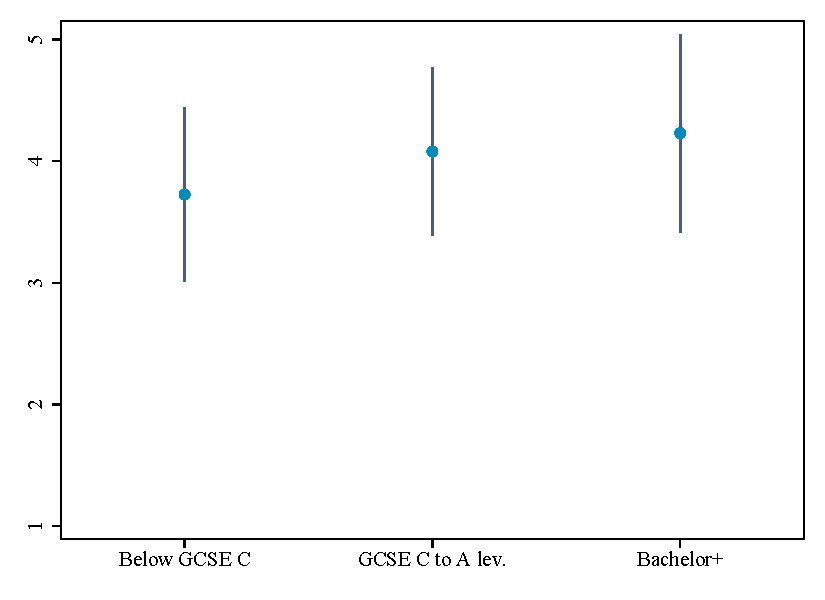
\includegraphics[width=.5\textwidth]{../output/routinepcuseCont1}} \subfloat[GCSE C-A levels]{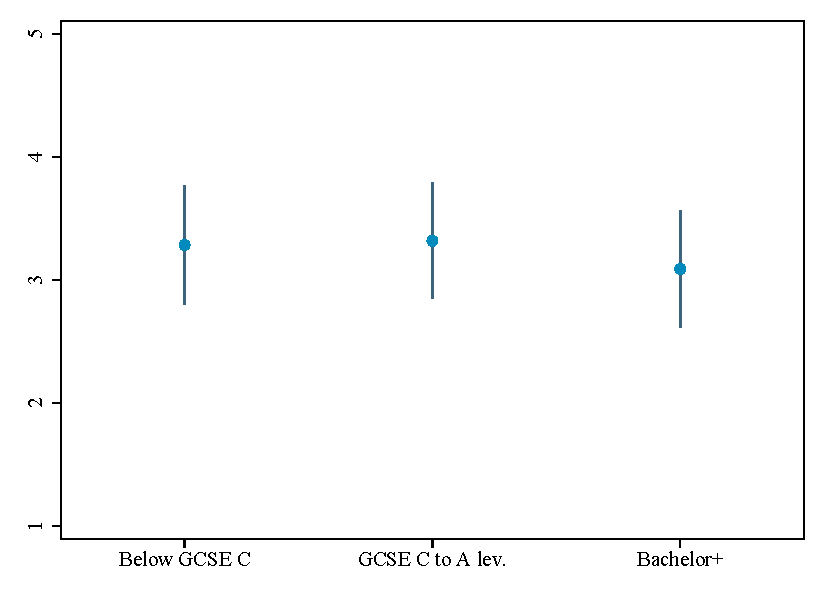
\includegraphics[width=.5\textwidth]{../output/routinepcuseCont2}} \\ \subfloat[Bachelor+]{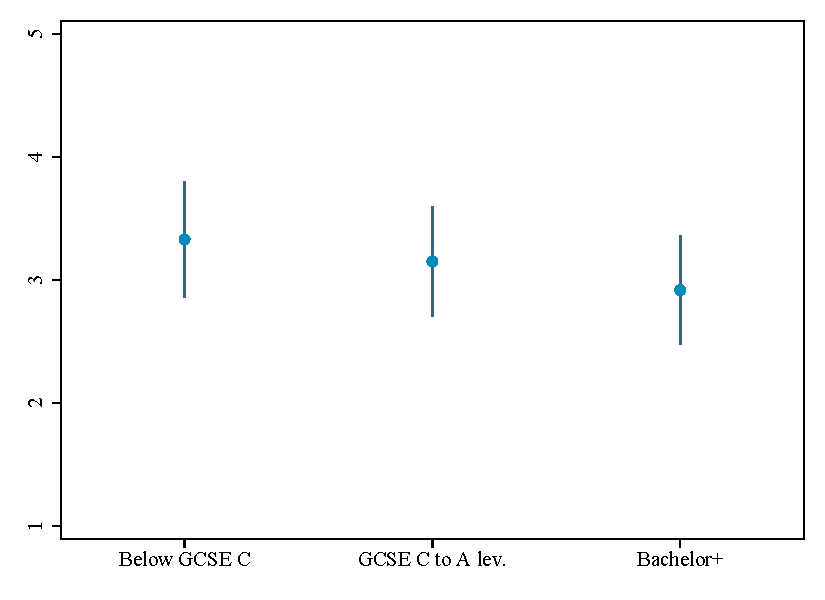
\includegraphics[width=.5\textwidth]{../output/routinepcuseCont3}} \subfloat[Below GCSE C/GCSE C-A levels]{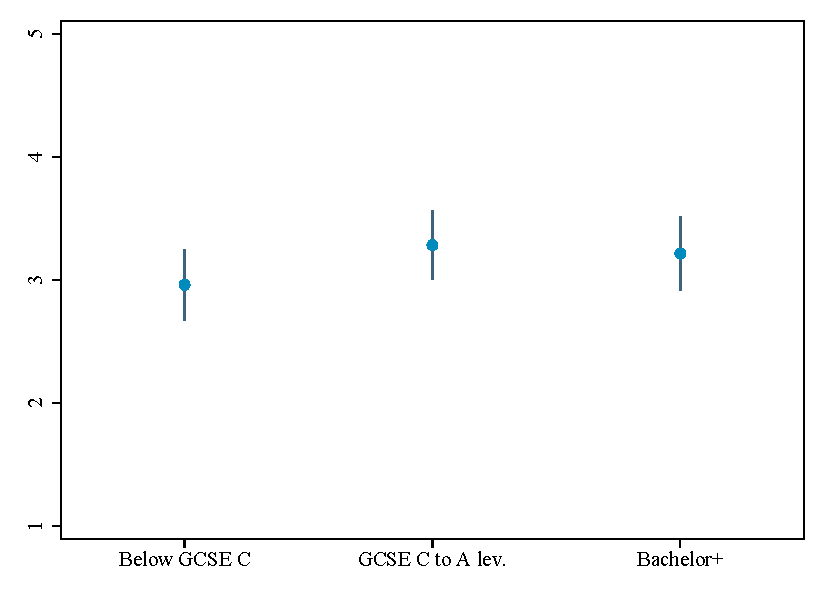
\includegraphics[width=.5\textwidth]{../output/routinepcuseCont12}} \\ \subfloat[GCSE C-A levels/Bachelor+]{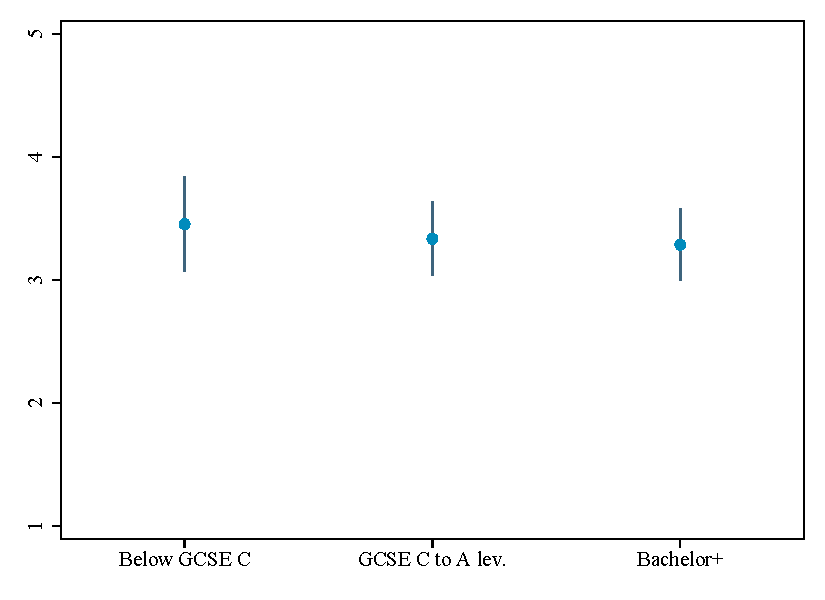
\includegraphics[width=.5\textwidth]{../output/routinepcuseCont23}} 
\par \begin{minipage}[h]{\textwidth}{\scriptsize\textbf{Note:} graphs show regression coefficients. Regressions include occupation and year fixed effects. CI based on robust standard errors. Higher values indicate less complex pc use. I assign a value of 1 to people who do not use a computer. Figure generated on 12 Jun 2020 at 15:40:43. Figure generated using the dofile 3\_sesAnalysis/pcUseTables.do.}\end{minipage}
\end{figure}
